
\chapter{Novel Approach: Reprojection
Mapping}\label{novel-approach-reprojection-mapping}

\section{Idea}\label{idea}

With the Reprojection method, a radar echo's source can be determined
without scanning the radar sensor. The distance to a target is already
available in the radar data, so only the direction is needed to update a
map. Under certain circumstances, this direction can also be extracted
from the sensor's data.

The prerequisite to the method is that the sensor has to move with a
known speed \(v_R\) through an otherwise static environment. Caused by
the radar's motion, the distance to all visible targets changes, which
causes a Doppler speed \(v_D\) for every target point.

\subsection{Geometry for the side-facing
case}\label{geometry-for-the-side-facing-case}

If the radar is moving directly towards a target, the target's Doppler
speed \(v_D\) will be equal to radar speed \(v_R\) (target \(A\) in
figure). If the radar passes the target on the side, so that the
distance to the target stops decreasing and begins to grow, \(v_D = 0\)
(target \(C\) in figure). If a target has an absolute Doppler speed
\(\|v_D\|\) between \(0\) and \(v_R\) (target \(B\) in figure), it is seen
from the radar under an angle \(\alpha\), such that
\[v_D = v_R cos(\alpha)\]

\begin{figure}
\centering
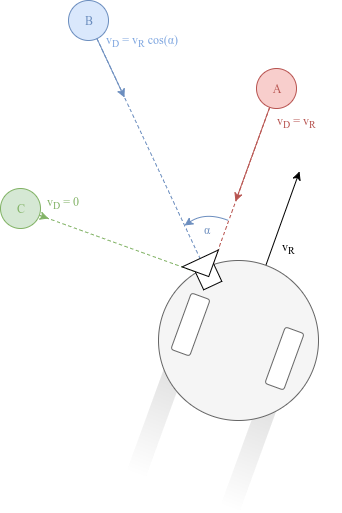
\includegraphics[width=0.5\textwidth]{diagrams/Radar_Reprojection_Geometry.png}
\caption{restrict-height}
\end{figure}

Positive values for \(\alpha\) indicate targets on the left side of the
robot, while negative values for \(\alpha\) indicate right hand side
targets. The caveat is that from \(v_D\) only the absolute value of
angle \(\alpha\) is known. This is OK if the radar is mounted
side-facing, such that only targets on one side of the motion path are
visible. Like this, the angle ambiguity is resolved, because only one
side is visible.

\subsection{Geometry for the General
case}\label{geometry-for-the-general-case}

In the general case such as with a forward facing radar, or with radar
antennas with angle sensitivities that allow a field of view of over
\(180^\circ\), the angle ambiguity must be resolved differently.

\begin{figure}
\centering
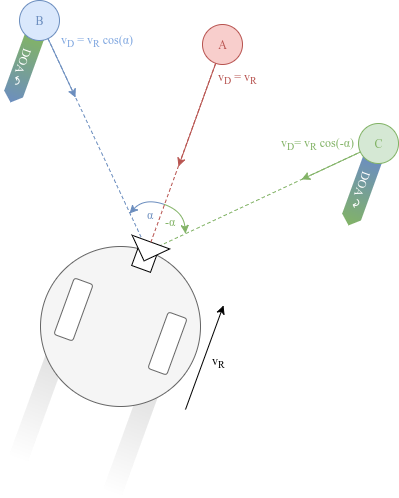
\includegraphics[width=0.5\textwidth]{diagrams/Radar_Reprojection_Geometry_forward.png}
\caption{restrict-height}
\end{figure}

One solution to resolving the angle ambiguity is to use direction of
arrival (DOA) information from a multistatic radar. If the radar is
facing straight forward, a target's DOA will be lower or higher,
depending on the antenna configuration and the side the target is being
passed on. If the radar is not facing straight but still has parts of
both sides of the motion paths visible in it's FOV the DOA gradient
should be used instead of its value: If a target's DOA is gradually
shifting towards left (i.e.~lower or higher, depending on the system),
it will pass the radar on the left side. If it is gradually shifting
towards right, it will pass on the right side.

\subsection{Reprojection Method}\label{reprojection-method}

TODO

When a target's range and angle are known, it can be mapped in relation
to the radar's position.

This allows intelligent path planning and obstacle avoidance for mobile
robots.



\subsection{Peak Gradient algorithm}\label{peak-gradient-algorithm}

TODO

One pillar of the Reprojection Method is the Doppler speed of static
targets. If the Doppler speed is not precisely measured, the
reprojection angle \(\alpha\) is imprecise or noisy, which leads to
smeared-out targets or even false positive detections on the map.

With FMCW radar, a target's range and Doppler speed can be
simultaneously registered.

\subsection{Limitations}\label{limitations}


TODO
